\documentclass[a4paper]{article}
\usepackage{amsfonts}



%% Language and font encodings
\usepackage[english]{babel}
\usepackage[utf8x]{inputenc}
\usepackage[T1]{fontenc}
\usepackage{graphicx,xcolor,colortbl}    
%% Sets page size and margins
\usepackage[a4paper,top=3cm,bottom=2cm,left=3cm,right=3cm,marginparwidth=1.75cm]{geometry}

%% Useful packages
\usepackage{amsmath}
\usepackage{graphicx}
\usepackage[colorinlistoftodos]{todonotes}
\usepackage[colorlinks=true, allcolors=blue]{hyperref}

\title{A python implementation of the Fully Bayesian Unfolding}
\author{Davide Gerbaudo, Clement Helsens, Francesco Rubbo}
% Shorthand for \phantom to use in tables
\newcommand{\pho}{\phantom{0}}
\newcommand{\bslash}{\ensuremath{\backslash}}
\newcommand{\BibTeX}{{\sc Bib\TeX}}
\newcommand{\Nl}{\mbox{$N_{\rm{loose}}$}}
\newcommand{\Nt}{\mbox{$N_{\rm{tight}}$}}
\newcommand{\Ns}{\mbox{$N^{\rm{SIG}}$}}
\newcommand{\Nf}{\mbox{$N^{\rm{FAKE}}$}}
\newcommand{\epss}{\mbox{$\varepsilon^{\rm{SIG}}$}}
%\newcommand{\epsf}{\mbox{$\varepsilon^{\rm{FAKE}}$}}
\newcommand{\zmumu}{\mbox{$\rm{Z}^0 \rightarrow \mu \mu$}~}
\newcommand{\zee}{\mbox{$\rm{Z}^0 \rightarrow e e$}~}
\newcommand{\ZZero}{\mbox{$\rm{Z}^0$}~}
\newcommand{\MTW}{\mbox{$M_{\rm{T}}(\rm{W})$}~}
\newcommand{\ljets}{\ensuremath{\ell{}+\text{jets}}}
\newcommand{\ejets}{\ensuremath{e+\text{jets}}}
\newcommand{\mujets}{\ensuremath{\mu{}+\text{jets}}}
\newcommand{\lumi}{\ensuremath{20.3~\ifb{}}}
\def\etconetwenty{\ensuremath{E_{T}^{0.2}}}
\def\etconethirty{\ensuremath{E_{T}^{0.3}}}
\def\ptconethirty{\ensuremath{p_{T}^{0.3}}}
\newcommand{\mymet}   {\ensuremath{E_{\mathrm{T}}^{\mathrm{miss}}}}
\newcommand{\etmiss}{$E_{\mathrm{T}}^{\mathrm{miss}}$}
%hypenated typewriter fonts 
% (see 
% http://tex.stackexchange.com/questions/44361/how-to-automatically-hyphenate-within-texttt )
\newcommand\hyptexttt[1]{\texttt{\hyphenchar\font=45\relax #1}}
% % Sub/superscript roman not italic (EE)
\def\MEX{\ensuremath{E_{\mathrm{x}}^{\mathrm{miss}}}}
\def\mex{\ensuremath{E_{\mathrm{x}}^{\mathrm{miss}}}}
\def\MEY{\ensuremath{E_{\mathrm{y}}^{\mathrm{miss}}}}
\def\mey{\ensuremath{E_{\mathrm{y}}^{\mathrm{miss}}}}
\def\MEXY{\ensuremath{E_{\mathrm{x,y}}^{\mathrm{miss}}}}
\def\mexy{\ensuremath{E_{\mathrm{x,y}}^{\mathrm{miss}}}}
\def\MEXYTRUTH{\ensuremath{E_{\mathrm{x,y Truth}}^{\mathrm{miss}}}}
\def\mexytruth{\ensuremath{E_{\mathrm{x,y Truth}}^{\mathrm{miss}}}}
\def\METTRUTH{\ensuremath{E_{\mathrm{T Truth}}^{\mathrm{miss}}}}
\def\mettruth{\ensuremath{E_{\mathrm{T Truth}}^{\mathrm{miss}}}}
% generators and formatting
\newcommand{\formatGenerator}[1]{\textsc{#1}}
\newcommand{\herwig}{\formatGenerator{herwig}}
\newcommand{\powheg}{\formatGenerator{powheg}}
\newcommand{\mcatnlo}{\formatGenerator{mcatnlo}}
\newcommand{\pythia}{\formatGenerator{pythia}}
\newcommand{\pythiaSix}{\formatGenerator{pythia~6}}
\newcommand{\alpgen}{\formatGenerator{alpgen}}
\newcommand{\athena}{\formatGenerator{athena}}
\newcommand{\mcnlo}{\formatGenerator{mc@nlo}}
\newcommand{\sherpa}{\formatGenerator{sherpa}}
\newcommand{\acermc}{\formatGenerator{acermc}}
\newcommand{\protos}{\formatGenerator{protos}}
\newcommand{\geantFour}{\formatGenerator{geant4}}
\newcommand{\jimmy}{\formatGenerator{jimmy}}
\newcommand{\hathor}{\formatGenerator{hathor}}
\newcommand{\atlfastTwo}{\formatGenerator{atlfast2}}
\newcommand{\wikiPage}[1]{\texttt{#1} wiki page}
% samples
\newcommand{\ttH}{\ensuremath{t\bar{t}H}}
\newcommand{\wjets}{\ensuremath{W+\mathrm{jets}}}
\newcommand{\wbb} {\ensuremath{Wb\bar{b}+{\rm jets}}}
\newcommand{\wcc} {\ensuremath{Wc\bar{c}+{\rm jets}}}
\newcommand{\wc} {\ensuremath{Wc+{\rm jets}}}
\newcommand{\wlight} {\ensuremath{W+{\rm light~jets}}}
\newcommand{\zjets}{\ensuremath{Z+\mathrm{jets}}}
% matrix method
\newcommand{\effFake}{\ensuremath{\epsilon_{\mathrm{fake}}}}
\newcommand{\effReal}{\ensuremath{\epsilon_{\mathrm{real}}}}
% Analysis variables
\newcommand{\qg}{\ensuremath{qg}}
\newcommand{\AC}{\ensuremath{\text{A}_{\text{C}}}}
\newcommand{\ACsub}[1]{\ensuremath{\text{A}_{\text{C}, #1}}}
\newcommand{\Et}{\ensuremath{E_{\text{T}}}}
%\newcommand{\pT}{\ensuremath{p_{\text{T}}}} % already defined in atlasphysics.sty
\newcommand{\ptSub}[1]{\ensuremath{p_{\text{T} #1}}}
\newcommand{\ptSup}[1]{\ensuremath{p_{\text{T}}^{#1}}}
\newcommand{\ptEl}{\ensuremath{p_{\text{T}}^{e}}}
\newcommand{\ptMu}{\ensuremath{p_{\text{T}}^{\mu{}}}}
%\newcommand{\met}{\ensuremath{\cancel{E}_{\text{T}}}} % already defined atlasphysics.sty
\newcommand{\mt}{\ensuremath{M_{\text{T}}}}
\newcommand{\mtw}{\ensuremath{M_{\text{T,W}}}}
%\newcommand{\ttbar}{\ensuremath{t\bar{t}}} % already defined atlasphysics.sty
\newcommand{\mtt}{\ensuremath{m_{\ttbar{}}}}
\newcommand{\pttt}{\ensuremath{p_{\text{T},\ttbar{}}}}
\newcommand{\ytt}{\ensuremath{y_{\ttbar{}}}}
\newcommand{\absYtt}{\ensuremath{\abs{y_{\ttbar{}}}}}
\newcommand{\betatt}{\ensuremath{\beta_{z,\ttbar{}}}}
\newcommand{\pp}{\ensuremath{pp}}
\newcommand{\ppbar}{\ensuremath{p\bar{p}}}
\newcommand{\deltaR}[2]{\ensuremath{\Delta{}R\left(#1, #2\right)}}
% FBU-related
\providecommand{\abs}[1]{\lvert#1\rvert} 
\newcommand{\dy}{\ensuremath{\Delta{}\abs{y}}}
\newcommand{\diffVar}{\ensuremath{\varv{}}}
\newcommand{\vect}[1]{\boldsymbol{#1}}
\newcommand{\thetavec}{\ensuremath{\vect{\theta{}}}}
\newcommand{\Truth}{\ensuremath{\vect{T}}}
\newcommand{\Data}{\ensuremath{\vect{D}}}
\newcommand{\Bckg}{\ensuremath{\vect{B}}}
\newcommand{\Reco}{\ensuremath{\vect{R}}}
\newcommand{\TrasfMatrix}{\ensuremath{\mathcal{M}}}
\newcommand{\Real}{\ensuremath{\mathbb{R}}}
\newcommand{\Integer}{\ensuremath{\mathbb{N}}}
\newcommand{\conditionalProb}[2]{\ensuremath{p\left(#1|#2\right)}}
\newcommand{\conditionalLhood}[2]{\ensuremath{\mathcal{L}\left(#1|#2\right)}}
\newcommand{\prior}{\ensuremath{\pi{}\left(\Truth{}\right)}}
\newcommand{\Tinf}{\ensuremath{T\ulcorner{}}}
\newcommand{\Tsup}{\ensuremath{T\urcorner{}}}
%\DeclareMathOperator{\Erf}{Erf}
%------------
% other various commands
%------------
%
% redefine marginpar (with tighter spacing)
\let\oldmarginpar\marginpar
\renewcommand\marginpar[1]{
  \-\oldmarginpar[\raggedleft\footnotesize #1]{\raggedright\footnotesize #1}
}

%------------
%
%------------


\begin{document}
\maketitle
\tableofcontents

\begin{abstract}
This document presents the python implementation of the Fully Bayesian Unfolding (FBU) method.
\end{abstract}

\section{Introduction}

The unfolding procedure is used to estimate a true spectrum
from the one measured in data. An observed spectrum is unfolded using
the fully bayesian unfolding (FBU) technique described in Ref.~\cite{Fbu2012arXiv1201.4612C}. 
We use the open-source \href{https://pypi.python.org/pypi/fbu}{PyFBU} 
implementation of the algorithm. 
The following sections provide an overview of the
method and a description of the possibilities this method allows.

\section{Goal of this paper}

\section{FBU ingredients}
The FBU method consists in the strict
application of Bayesian inference to the problem of unfolding. This
application can be stated in the following terms: given an observed
spectrum $\Data\in\Integer^{N_r}$ and a response matrix
$\TrasfMatrix\in\Real{}^{N_r}\times{}\Real{}^{N_t}$, the posterior
probability of the true spectrum $\Truth{}\in{}\Real{}^{N_t}$ follows
the probability density
\begin{equation}
\conditionalProb{\Truth{}}{\Data{},\TrasfMatrix{}}
\propto{}
\conditionalLhood{\Data{}}{\Truth{},\TrasfMatrix{}}
\cdot{}
\pi{}\left(\Truth{}\right)
\end{equation}
where \conditionalLhood{\Data{}}{\Truth{},\TrasfMatrix{}} is the
likelihood function of \Data{} given \Truth{} and \TrasfMatrix{},
and $\pi{}$ is the prior probability density for the true spectrum
\Truth{}.
Each of these ingredients is described in the following.

\subsection{Likelihood}
\label{sec:fbullhood}
Under the assumption that the data are poissonian counts, the
likelihood \conditionalLhood{\Data{}}{\Truth{},\TrasfMatrix{}} can be
computed from the following two pieces of information, contained in
the response matrix \TrasfMatrix{}:
\begin{itemize}
\item the probability $P(r_i|t_j)$ for an event produced in the true bin
$t_j$ to be observed in the reconstructed bin $r_i$;
\item the efficiency $\epsilon{}_{t_j}$ for an event produced in the
true bin $t_j$ to be reconstructed in any bin $r$.
\end{itemize}
The above quantities define the elements
$m_{ij}=\epsilon_{t_j}\cdot{}p(r_i|t_j)$ of \TrasfMatrix{}, and allow
the prediction of the reconstructed spectrum $\vect{R}$ corresponding to
a given true spectrum \Truth{} as given by
\begin{equation}
r_i(\Truth{},\TrasfMatrix{}) = \sum_{j=0}^{N_r}m_{ij}\cdot{}t_j.
\end{equation}
The likelihood is then defined by comparing the observed spectrum
\Data{} with the expected one, which includes the background
prediction $\vect{B}$:
\begin{equation}
\label{eq:lhood}
\conditionalLhood{\Data{}}{\Truth{},\TrasfMatrix{},\vect{B}} =
\prod_{i=1}^{N_r}Poisson(d_i,r_i(\Truth{},\TrasfMatrix{})+b_i).
\end{equation}

\subsection{Prior}
\label{sec:fbuprior}
While the response matrix can be estimated from the simulated
sample of signal events, the prior probability density \prior{} is to
be chosen according to what we know about \Truth{} before the
measurement is performed.
The simplest choice is an {\it uninformative}
prior that assigns equal probabilities to all \Truth{} spectra within
a wide range $\left[\Tinf{}, \Tsup{}\right]$:
\begin{equation}
\prior{}
\propto{}
\begin{cases}
1 & \text{if }
T_{t}\in{}\left[\Tinf{}, \Tsup{}\right], \forall{}t\in{}\left[1, N_t\right] \\
0 & \text{otherwise} \\
\end{cases}
\end{equation}
A more general definition for the prior is given by
\begin{equation}
\prior{}
\propto{}
\begin{cases}
e^{\alpha{}S(\Truth{})} & \text{if }
T_{t}\in{}\left[\Tinf{}, \Tsup{}\right], \forall{}t\in{}\left[1, N_t\right] \\
0 & \text{otherwise} \\
\end{cases}
\end{equation}
where $\alpha{}$ is an arbitrary strength parameter, and
$S(\Truth{})$ is a regularization function.
The choice of $\alpha$ determines the impact of the prior on
\conditionalProb{\Truth{}}{\Data{}}, while $S(\Truth{})$ determines
what additional information is being used to constrain the parameter
space, thus reducing the variance of the \Truth{} parameters by
introducing a small bias.
In the analysis, the uninformative
prior is used for all measurements.

\subsection{Sampling}
\label{subsec:sampling}
Having chosen the prior, the posterior probability density 
$\conditionalProb{\Truth{}}{\Data{}}$ is determined by 
sampling the $N_t$-dimensional parameter space, 
and evaluating for each point $\conditionalLhood{\Data{}}{\Truth{}}$ and
\prior{}, thus performing a numerical integration. 
For a large number of parameters, direct sampling techniques 
become extremely inefficient. Therefore, the Metropolis-Hastings algorithm~\cite{Metropolis:1953am}, 
a Markov Chain Monte Carlo (MCMC) method~\cite{Markov} 
specialized for multi-dimensional sampling, is used for FBU. Combining this set of points with the 
weight given by $\conditionalLhood{\Data{}}{\Truth{},\TrasfMatrix{}} \cdot \pi$, 
one can determine the posterior probability density distribution 
for each bin of the spectrum, as well as for any quantity that is 
computed from the spectrum, such as $\AC{}$:
\begin{equation}
\conditionalProb{\AC{}}{\Data{}} = \int{ \delta(\AC{} - \AC{}(\Truth{})) \conditionalProb{\Truth{}}{\Data{}} d \Truth{}} 
\end{equation}

\subsection{Multi-dimensional unfolding}
\label{subsec:unf:twodim}
The same setup used for the one-dimensional unfolding can also be used to unfold multi-dimensional distributions, in which the other dimensions
corresponds to the bins of the differential variable  $\nu$ ,
where $\nu$ can be any differential variable. The spectrum
formatting, however, is different in that the multi-dimensional
histogram is transformed into a one-dimensional histogram. The other
dimensions of the multi-dimensional histogram is wrapped as several
consecutive sub-ranges of the first dimension.


\subsection{Marginalization}
\label{sec:marginalization}
The treatment of systematic uncertainties is naturally included in the
Bayesian inference approach by extending the likelihood
\conditionalLhood{\Data{}}{\Truth{}} with nuisance parameters terms.
The {\it marginal} likelihood is defined as
\begin{equation}
\conditionalLhood{\Data{}}{\Truth{}}=
\int
\conditionalLhood{\Data{}}{\Truth{},\thetavec{}}
\cdot{} \pi{}(\thetavec{})
~d\thetavec{},
\end{equation}
where \thetavec{} are the nuisance parameters, and
$\pi{}(\thetavec{})$ their prior probability densities, which are
assumed to be Gaussian distributions $G$ with $\mu=0$ and $\sigma=1$.
A nuisance parameter is associated with each of the uncertainty sources. 
Two categories of nuisances are considered: 
the normalizations of the background processes
($\thetavec{}_b$), and the uncertainties associated to the objects
identification, reconstruction and calibration ($\thetavec{}_s$).
While the first ones only affect the background predictions, the
latter, referred to as object systematic uncertainties, affect both the
reconstructed distribution for signal and
the total background prediction, referred to as
$\Reco{}(\Truth{};\thetavec{}_s)$ and
$\Bckg{}(\thetavec{}_s,\thetavec{}_b)$, respectively.
The marginal likelihood becomes then
\begin{equation}
\label{eq:marginalLhood}
\conditionalLhood{\Data{}}{\Truth{}}=
\int
\conditionalLhood{\Data{}}{\Reco{}(\Truth{};\thetavec{}_s),\Bckg{}(\thetavec{}_s,\thetavec{}_b)}
\cdot{} G(\thetavec{}_s) ~G(\thetavec{}_b)
~d\thetavec{}_s ~d\thetavec{}_b.
\end{equation}
The differential likelihood
$\conditionalLhood{\Data{}}{\Reco{}(\Truth{};\thetavec{}_s),\Bckg{}(\thetavec{}_s,\thetavec{}_b)}$
is defined as in Eq.~\ref{eq:lhood}, with
\begin{equation}
r_i(\Truth{},\TrasfMatrix{};\thetavec{}_s) =
r_i(\Truth{},\TrasfMatrix{};0) \cdot ( 1 + \sum_k
\theta_s^k\cdot\Delta r_i^k )
\end{equation}
and, for each background process $b$,
\begin{equation}
b_i(\thetavec{}_s,\theta_b) =
b_i(0) \cdot ( 1 + \theta_b\cdot\Delta b) \cdot
(1 + \sum_k \theta_s^k\cdot\Delta b_i^k ),
\end{equation}
where $r_i(\Truth{},\TrasfMatrix{};0)$ and $b_i(0)$ represent the
nominal reconstructed--level signal and background
predictions, respectively;
$\Delta b$ is the uncertainty on the background normalization;
$\Delta r_i^k$ and $\Delta b_i^k$ are the systematic variations for
the signal and background, respectively, in
bin $i$, corresponding to the uncertainty $k$, and the sum runs over
all sources of object systematic uncertainty.
The prior probability densities $G(\thetavec{}_b)$ are truncated at
$\theta_{min}=-1/\Delta b$ in order to avoid negative background
normalizations. 
The truncation affects only the backgrounds with large normalization 
uncertainty. 
None of these should impact the measurement significantly and it in any case should be checked that the truncation does not change the behavior of the marginalization
procedure (As it has been done for ATLAS published analyses)

The marginal posterior probability density for \Truth{} is computed by
sampling the $N_t+N_{np}$ parameter space, where $N_{np}$ is the
total number of nuisance parameters, and projecting the sample over
the \Truth{} parameter space. The projections over each nuisance
parameter give the corresponding posterior probability density,
which matches the Gaussian prior for unconstrained nuisance
parameters, while it has a narrower shape for nuisance parameters
that can be measured in the dataset (see Fig.~\ref{fig:nuisparpost}).
The posterior probability density for \AC{} is computed as described in
Sec.~\ref{subsec:sampling} with the difference that the RMS of the
marginal posterior represents the total uncertainty. Analogously, each
nuisance parameter is estimated by the mean and RMS of the
corresponding projection of the posterior probability density.
\begin{figure}[!htb]\centering
Sanity checks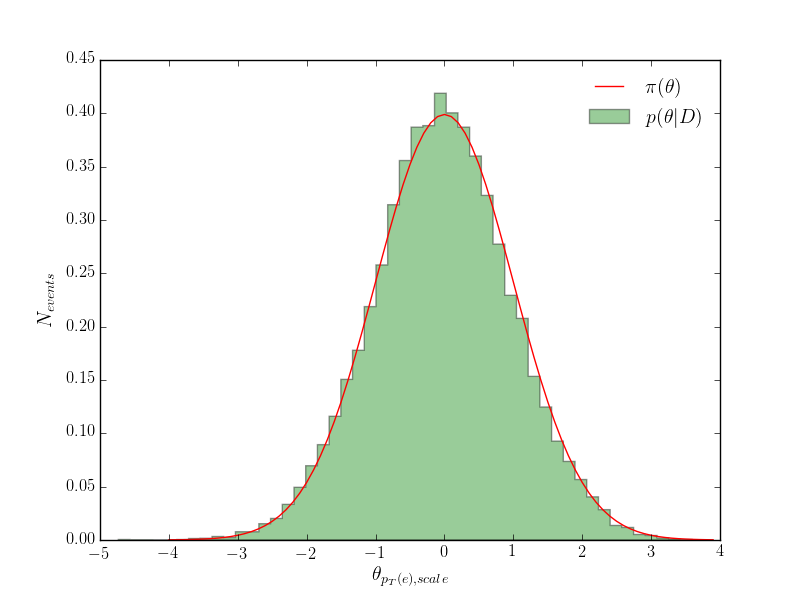
\includegraphics[width=0.495\textwidth]{unconstrainednp.png}
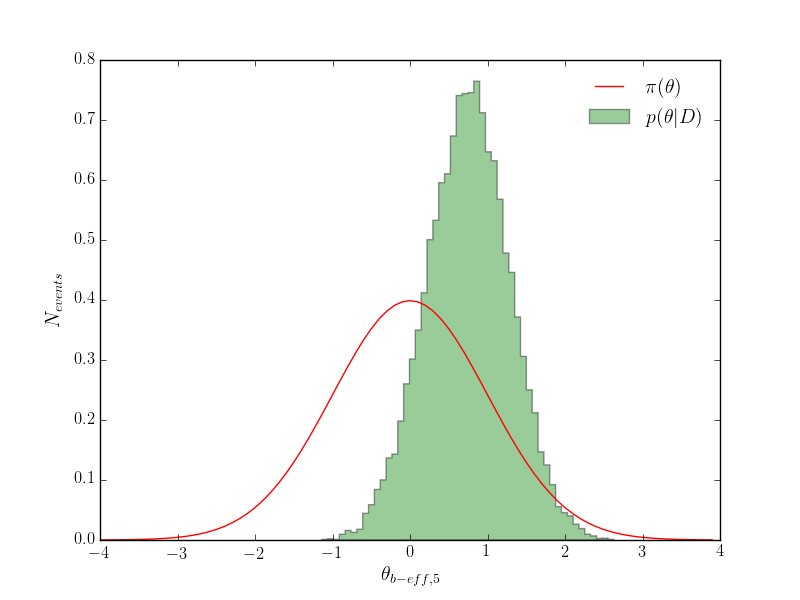
\includegraphics[width=0.495\textwidth]{constrainednp.png}
\caption{Prior and posterior probability densities for nuisance parameters
corresponding to a nuisance parameter that has no constraining power(left) and a
nuisance parameter that has some constraining power (right).}
\label{fig:nuisparpost}
\end{figure}



\subsection{Combination of channels}
\label{sec:chcomb}
As discussed in Sec.~\ref{sec:wjets}, the combination of
orthogonal channels with different background compositions is crucial
to estimate precisely the \wjets{} contamination in the
data sample. 
The marginalization approach provides a natural framework to treat
simultaneously unfolding and background estimation using
multiple data regions. Given the distributions $\Data{}_i$ measured in $N_{ch}$
independent channels, the likelihood defined in Eq.~\ref{eq:marginalLhood}
is extended to the product of likelihoods of each channel, so that
\begin{equation}
\conditionalLhood{\{\Data{}_1\cdots{}\Data{}_{N_{ch}}\}}{\Truth{}}=
\int
\prod_{i=1}^{N_{ch}}\conditionalLhood{\Data{}_i}{\Truth{};\thetavec{}}
\cdot{} G(\thetavec{})
~d\thetavec{},
\end{equation}
where the nuisance parameters are common to all analysis channels.
are free parameters in the likelihood.
The constraint on the $W^{+}/W^{-}$ enters in the likelihood 
through the channels combination so the K factors are independent 
of the charge and so by fitting both charges during marginalization, we
 are sensitive to the values of the different K


The posterior probability density is thus
\begin{equation}
\begin{split}
\conditionalProb{\Truth{}}{\{\Data{}_1\cdots{}\Data{}_{N_{ch}}\}}=&
\int
\prod_{i=1}^{N_{ch}}\conditionalLhood{\Data{}_i}{\Reco{}_i(\Truth{};\thetavec{}_s),\Bckg{}_i(K_{1},K_c,K_{light};\thetavec{}_s,\thetavec{}_b)}\\
& ~G(\thetavec{}_s)
~G(\thetavec{}_b)
~\pi{}(\Truth{})
~\pi{}(K_{1})
~\pi{}(K_c)
~\pi{}(K_{light})
~d\thetavec{}_s
~d\thetavec{}_b,\\
\end{split}
\end{equation}
with
$\Bckg{}=\Bckg{}(K_{1},K_c,K_{light};\thetavec_s,\thetavec{}_b)$,
and the $\pi{}$'s are uninformative priors.
A total of 53 object definition parameters $\thetavec_s$ are
considered, corresponding to the sources of systematic uncertainty
discussed in Sec.~\ref{sec:syst_objects}.
Eleven normalization nuisance parameters $\thetavec_b$ are considered
for the background processes other than \wjets{}: single top, \zjets{}, diboson 
and multijet. Independent nuisance parameters are assigned to \zjets{}
and multijet normalizations for each $b$--jet multiplicity, given that
the modeling of $b$--tagging efficiencies is not calibrated
specifically for these processes. Independent nuisance parameters are
considered for the multijet background estimation in \mujets{} and in
\ejets{}. An additional normalization parameter $\theta_{Luminosity}$,
corresponding to the uncertainty on the integrated luminosity to which
the MC samples are normalized, is assigned to the simulated single
top, \zjets{} and diboson backgrounds.
Figure~\ref{fig:nuispar} summarizes the expected precision and measured
values for all nuisance parameters. The expected precision is obtained
by evaluating the likelihood for a pseudo--data sample corresponding
to the sum of background and signal predictions; thus the central
value for each parameter is measured to be $\theta\sim0$, while the
uncertainty is $\delta\theta\leq1$, depending on the constraining power of
the dataset on each parameter.
\begin{figure}[!htb]\centering
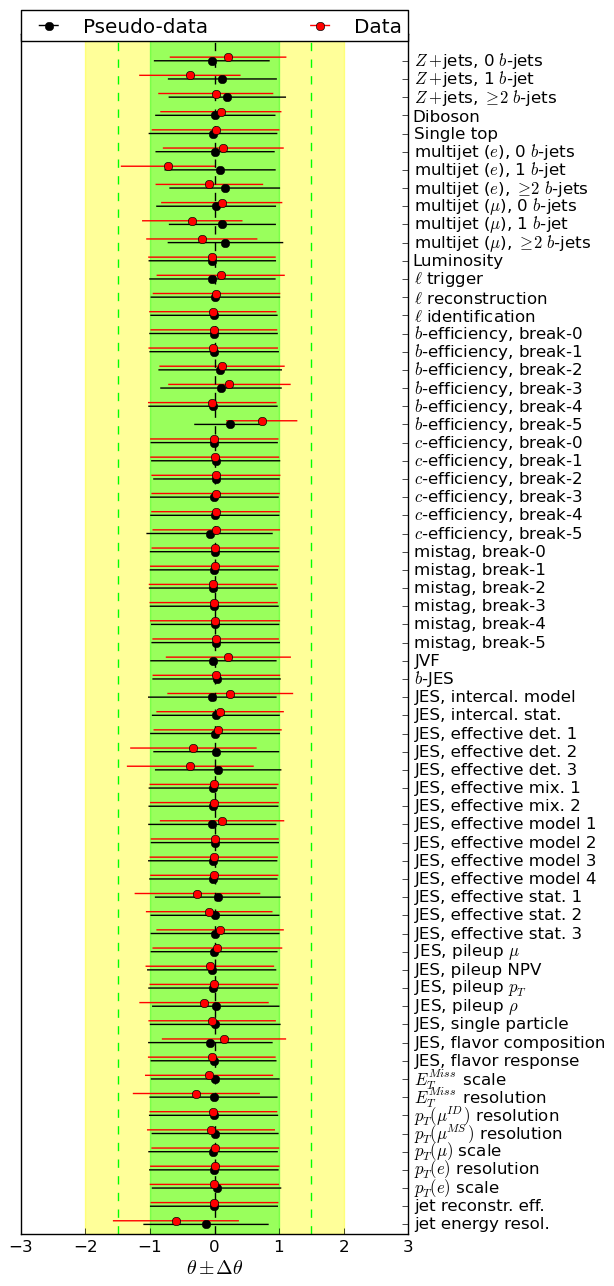
\includegraphics[width=0.6\textwidth]{nuispar}
\caption{The mean and RMS of the posterior probability density for
each nuisance parameter in pseudo--data (black) and data
(red) are shown for the inclusive \AC{} measurement. The
shaded regions highlight the $1\sigma$ (green) and $2\sigma$
intervals of the prior probability density.}
\label{fig:nuispar}
\end{figure}
The likelihood evaluated for the actual data gives the nuisance
parameters corresponding to the measurements.
Most nuisance parameters are measured to be well within $1\sigma$ of
their prior probability density, with little constraining power
($\delta\theta\approx1$). The $b$--jet multiplicity provides
information on the $b$--tag calibration, whose largest uncertainty
component ($b$--efficiency, break--5) is constrained. The nuisance
parameters for the measurement as a function of mtt and a
comparison of e+jets and mu+jets channels is shown in
App.~\ref{sec:app:unfolding:marginalization}.


\section{Implementation}
The python programming language was used to implement the FBU method within a user friendly setup. It is done in the \href{https://pypi.python.org/pypi/fbu}{PyFBU} implementation described in this paper has already been used in four published results of the ATLAS collaboration using proton-proton collision data provided by the CERN Large Hadron Collider (LHC)~\cite{Aad:2015noh,Aad:2015lgx,Aad:2016ove,Aaboud:2016bit}.

\section{Sanity checks}

\bibliographystyle{unsrt}
\bibliography{bibliography.bib}


\end{document}